\documentclass[a4paper]{article}

\def\npart {IB}
\def\nterm {Michaelmas}
\def\nyear {2015}
\def\nlecturer {N. Wickramasekera}
\def\ncourse {Analysis II}
\def\nlectures {MWF.12}
\def\nnotready {}

% Imports
\ifx \nextra \undefined
  \usepackage[pdftex,
    hidelinks,
    pdfauthor={Dexter Chua},
    pdfsubject={Cambridge Maths Notes: Part \npart\ - \ncourse},
    pdftitle={Part \npart\ - \ncourse},
  pdfkeywords={Cambridge Mathematics Maths Math \npart\ \nterm\ \nyear\ \ncourse}]{hyperref}
  \title{Part \npart\ - \ncourse}
\else
  \usepackage[pdftex,
    hidelinks,
    pdfauthor={Dexter Chua},
    pdfsubject={Cambridge Maths Notes: Part \npart\ - \ncourse\ (\nextra)},
    pdftitle={Part \npart\ - \ncourse\ (\nextra)},
  pdfkeywords={Cambridge Mathematics Maths Math \npart\ \nterm\ \nyear\ \ncourse\ \nextra}]{hyperref}

  \title{Part \npart\ - \ncourse \\ {\Large \nextra}}
\fi

\author{Lectured by \nlecturer \\\small Notes taken by Dexter Chua}
\date{\nterm\ \nyear}

\usepackage{alltt}
\usepackage{amsfonts}
\usepackage{amsmath}
\usepackage{amssymb}
\usepackage{amsthm}
\usepackage{booktabs}
\usepackage{caption}
\usepackage{enumitem}
\usepackage{fancyhdr}
\usepackage{graphicx}
\usepackage{mathtools}
\usepackage{microtype}
\usepackage{multirow}
\usepackage{pdflscape}
\usepackage{pgfplots}
\usepackage{siunitx}
\usepackage{tabularx}
\usepackage{tikz}
\usepackage{tkz-euclide}
\usepackage[normalem]{ulem}
\usepackage[all]{xy}

\pgfplotsset{compat=1.12}

\pagestyle{fancyplain}
\lhead{\emph{\nouppercase{\leftmark}}}
\ifx \nextra \undefined
  \rhead{
    \ifnum\thepage=1
    \else
      \npart\ \ncourse
    \fi}
\else
  \rhead{
    \ifnum\thepage=1
    \else
      \npart\ \ncourse\ (\nextra)
    \fi}
\fi
\usetikzlibrary{arrows}
\usetikzlibrary{decorations.markings}
\usetikzlibrary{decorations.pathmorphing}
\usetikzlibrary{positioning}
\usetikzlibrary{fadings}
\usetikzlibrary{intersections}
\usetikzlibrary{cd}

\newcommand*{\Cdot}{\raisebox{-0.25ex}{\scalebox{1.5}{$\cdot$}}}
\newcommand {\pd}[2][ ]{
  \ifx #1 { }
    \frac{\partial}{\partial #2}
  \else
    \frac{\partial^{#1}}{\partial #2^{#1}}
  \fi
}

% Theorems
\theoremstyle{definition}
\newtheorem*{aim}{Aim}
\newtheorem*{axiom}{Axiom}
\newtheorem*{claim}{Claim}
\newtheorem*{cor}{Corollary}
\newtheorem*{defi}{Definition}
\newtheorem*{eg}{Example}
\newtheorem*{fact}{Fact}
\newtheorem*{law}{Law}
\newtheorem*{lemma}{Lemma}
\newtheorem*{notation}{Notation}
\newtheorem*{prop}{Proposition}
\newtheorem*{thm}{Theorem}

\renewcommand{\labelitemi}{--}
\renewcommand{\labelitemii}{$\circ$}
\renewcommand{\labelenumi}{(\roman{*})}

\let\stdsection\section
\renewcommand\section{\newpage\stdsection}

% Strike through
\def\st{\bgroup \ULdepth=-.55ex \ULset}

% Maths symbols
\newcommand{\bra}{\langle}
\newcommand{\ket}{\rangle}

\newcommand{\N}{\mathbb{N}}
\newcommand{\Z}{\mathbb{Z}}
\newcommand{\Q}{\mathbb{Q}}
\renewcommand{\H}{\mathbb{H}}
\newcommand{\R}{\mathbb{R}}
\newcommand{\C}{\mathbb{C}}
\newcommand{\Prob}{\mathbb{P}}
\renewcommand{\P}{\mathbb{P}}
\newcommand{\E}{\mathbb{E}}
\newcommand{\F}{\mathbb{F}}
\newcommand{\cU}{\mathcal{U}}
\newcommand{\RP}{\mathbb{RP}}
\newcommand{\CP}{\mathbb{CP}}

\newcommand{\ph}{\,\cdot\,}

\DeclareMathOperator{\sech}{sech}
\DeclareMathOperator{\cosech}{cosech}
\DeclareMathOperator{\cosec}{cosec}

\DeclareMathOperator{\covol}{covol}
\DeclareMathOperator{\vol}{vol}

\let\Im\relax
\let\Re\relax
\DeclareMathOperator{\Im}{Im}
\DeclareMathOperator{\Re}{Re}
\DeclareMathOperator{\im}{im}
\DeclareMathOperator{\image}{image}
\DeclareMathOperator{\Ann}{Ann}

\DeclareMathOperator*{\res}{res}
\DeclareMathOperator{\Res}{Res}
\DeclareMathOperator{\Ind}{Ind}

\DeclareMathOperator{\tr}{tr}
\DeclareMathOperator{\diag}{diag}
\DeclareMathOperator{\rank}{rank}
\DeclareMathOperator{\card}{card}
\DeclareMathOperator{\spn}{span}
\DeclareMathOperator{\adj}{adj}

\DeclareMathOperator{\erf}{erf}
\DeclareMathOperator{\erfc}{erfc}

\DeclareMathOperator{\ord}{ord}
\DeclareMathOperator{\Sym}{Sym}

\DeclareMathOperator{\sgn}{sgn}
\DeclareMathOperator{\orb}{orb}
\DeclareMathOperator{\stab}{stab}
\DeclareMathOperator{\ccl}{ccl}

\DeclareMathOperator{\lcm}{lcm}
\DeclareMathOperator{\hcf}{hcf}

\DeclareMathOperator{\Int}{Int}
\DeclareMathOperator{\id}{id}

\DeclareMathOperator{\betaD}{beta}
\DeclareMathOperator{\gammaD}{gamma}
\DeclareMathOperator{\Poisson}{Poisson}
\DeclareMathOperator{\binomial}{binomial}
\DeclareMathOperator{\multinomial}{multinomial}
\DeclareMathOperator{\Bernoulli}{Bernoulli}
\DeclareMathOperator{\like}{like}

\DeclareMathOperator{\var}{var}
\DeclareMathOperator{\cov}{cov}
\DeclareMathOperator{\bias}{bias}
\DeclareMathOperator{\mse}{mse}
\DeclareMathOperator{\corr}{corr}

\DeclareMathOperator{\otp}{otp}
\DeclareMathOperator{\dom}{dom}

\DeclareMathOperator{\Root}{Root}
\DeclareMathOperator{\supp}{supp}
\DeclareMathOperator{\rel}{rel}
\DeclareMathOperator{\Hom}{Hom}
\DeclareMathOperator{\Aut}{Aut}
\DeclareMathOperator{\Gal}{Gal}
\DeclareMathOperator{\Mat}{Mat}
\DeclareMathOperator{\End}{End}
\DeclareMathOperator{\Char}{char}
\DeclareMathOperator{\ev}{ev}
\DeclareMathOperator{\St}{St}
\DeclareMathOperator{\Lk}{Lk}
\DeclareMathOperator{\disc}{disc}
\DeclareMathOperator{\Isom}{Isom}
\DeclareMathOperator{\length}{length}
\DeclareMathOperator{\energy}{energy}
\DeclareMathOperator{\area}{area}
\DeclareMathOperator{\Syl}{Syl}
\DeclareMathOperator{\cl}{cl}
\DeclareMathOperator{\fix}{fix}

\newcommand{\GL}{\mathrm{GL}}
\newcommand{\SL}{\mathrm{SL}}
\newcommand{\PGL}{\mathrm{PGL}}
\newcommand{\PSL}{\mathrm{PSL}}
\newcommand{\PSU}{\mathrm{PSU}}
\newcommand{\Or}{\mathrm{O}}
\newcommand{\SO}{\mathrm{SO}}
\newcommand{\U}{\mathrm{U}}
\newcommand{\SU}{\mathrm{SU}}

\renewcommand{\d}{\mathrm{d}}
\newcommand{\D}{\mathrm{D}}

\tikzset{->/.style = {decoration={markings,
                                  mark=at position 1 with {\arrow[scale=2]{latex'}}},
                      postaction={decorate}}}
\tikzset{<-/.style = {decoration={markings,
                                  mark=at position 0 with {\arrowreversed[scale=2]{latex'}}},
                      postaction={decorate}}}
\tikzset{<->/.style = {decoration={markings,
                                   mark=at position 0 with {\arrowreversed[scale=2]{latex'}},
                                   mark=at position 1 with {\arrow[scale=2]{latex'}}},
                       postaction={decorate}}}
\tikzset{->-/.style = {decoration={markings,
                                   mark=at position #1 with {\arrow[scale=2]{latex'}}},
                       postaction={decorate}}}
\tikzset{-<-/.style = {decoration={markings,
                                   mark=at position #1 with {\arrowreversed[scale=2]{latex'}}},
                       postaction={decorate}}}

\tikzset{circ/.style = {fill, circle, inner sep = 0, minimum size = 3}}
\tikzset{mstate/.style={circle, draw, blue, text=black, minimum width=0.7cm}}

\definecolor{mblue}{rgb}{0.2, 0.3, 0.8}
\definecolor{morange}{rgb}{1, 0.5, 0}
\definecolor{mgreen}{rgb}{0.1, 0.4, 0.2}
\definecolor{mred}{rgb}{0.5, 0, 0}

\def\drawcirculararc(#1,#2)(#3,#4)(#5,#6){%
    \pgfmathsetmacro\cA{(#1*#1+#2*#2-#3*#3-#4*#4)/2}%
    \pgfmathsetmacro\cB{(#1*#1+#2*#2-#5*#5-#6*#6)/2}%
    \pgfmathsetmacro\cy{(\cB*(#1-#3)-\cA*(#1-#5))/%
                        ((#2-#6)*(#1-#3)-(#2-#4)*(#1-#5))}%
    \pgfmathsetmacro\cx{(\cA-\cy*(#2-#4))/(#1-#3)}%
    \pgfmathsetmacro\cr{sqrt((#1-\cx)*(#1-\cx)+(#2-\cy)*(#2-\cy))}%
    \pgfmathsetmacro\cA{atan2(#2-\cy,#1-\cx)}%
    \pgfmathsetmacro\cB{atan2(#6-\cy,#5-\cx)}%
    \pgfmathparse{\cB<\cA}%
    \ifnum\pgfmathresult=1
        \pgfmathsetmacro\cB{\cB+360}%
    \fi
    \draw (#1,#2) arc (\cA:\cB:\cr);%
}
\newcommand\getCoord[3]{\newdimen{#1}\newdimen{#2}\pgfextractx{#1}{\pgfpointanchor{#3}{center}}\pgfextracty{#2}{\pgfpointanchor{#3}{center}}}

\def\Xint#1{\mathchoice
   {\XXint\displaystyle\textstyle{#1}}%
   {\XXint\textstyle\scriptstyle{#1}}%
   {\XXint\scriptstyle\scriptscriptstyle{#1}}%
   {\XXint\scriptscriptstyle\scriptscriptstyle{#1}}%
   \!\int}
\def\XXint#1#2#3{{\setbox0=\hbox{$#1{#2#3}{\int}$}
     \vcenter{\hbox{$#2#3$}}\kern-.5\wd0}}
\def\ddashint{\Xint=}
\def\dashint{\Xint-}


\begin{document}
\maketitle
{\small
\noindent\textbf{Uniform convergence}\\
The general principle of uniform convergence. A uniform limit of continuous functions is continuous.  Uniform convergence and termwise integration and differentiation of series of real-valued functions. Local uniform convergence of power series.\hspace*{\fill} [3]

\vspace{10pt}
\noindent\textbf{Uniform continuity and integration}\\
Continuous functions on closed bounded intervals are uniformly continuous. Review of basic facts on Riemann integration (from Analysis I). Informal discussion of integration of complex-valued and $\R^n$-valued functions of one variable; proof that $\|\int_a^b f(x) \;\d x\| \leq \int_a^b \|f(x)\|\;\d x$.\hspace*{\fill} [2]

\vspace{10pt}
\noindent\textbf{$\R^n$ as a normed space}\\
Definition of a normed space. Examples, including the Euclidean norm on $\R^n$ and the uniform norm on $\mathcal{C}[a, b]$. Lipschitz mappings and Lipschitz equivalence of norms. The Bolzano-Weierstrass theorem in $\R^n$. Completeness. Open and closed sets. Continuity for functions between normed spaces. A continuous function on a closed bounded set in $\R^n$ is uniformly continuous and has closed bounded image. All norms on a finite-dimensional space are Lipschitz equivalent.\hspace*{\fill} [5]

\vspace{10pt}
\noindent\textbf{Differentiation from $\R^m$ to $\R^n$}\\
Definition of derivative as a linear map; elementary properties, the chain rule. Partial derivatives; continuous partial derivatives imply differentiability. Higher-order derivatives; symmetry of mixed partial derivatives (assumed continuous). Taylor's theorem. The mean value inequality. Path-connectedness for subsets of $\R^n$; a function having zero derivative on a path-connected open subset is constant.\hspace*{\fill} [6]

\vspace{10pt}
\noindent\textbf{Metric spaces}\\
Definition and examples. *Metrics used in Geometry*. Limits, continuity, balls, neighbourhoods, open and closed sets.\hspace*{\fill} [4]

\vspace{10pt}
\noindent\textbf{The Contraction Mapping Theorem}\\
The contraction mapping theorem. Applications including the inverse function theorem (proof of continuity of inverse function, statement of differentiability). Picard's solution of differential equations.\hspace*{\fill} [4]}

\tableofcontents

\section{Uniform convergence}
Here we are concerned with sequences of functions. In general, let $E$ be any set, and $f_n: E\to \R$ for $n = 1, 2, \cdots$. Suppose for all $x\in E$, the sequence $(f_n(x))$ of real numbers converges (to some element in the real line).

We can define $f: E \to \R$ by $f(x) = \lim\limits_{n \to \infty} f_n(x)$. We say that $f_n$ converges \emph{pointwise} to $f$.

\begin{defi}[Pointwise convergence]
  The sequence $f_n$ converges \emph{pointwise} to $f$ if
  \[
    f(x) = \lim_{n\to \infty} f(x)
  \]
  for all $x$.
\end{defi}

Ideally, We want to deduce properties of $f$ from properties of $f_n$. For example, it would be great that continuity of all $f_n$ implies continuity of $f$, and similarly for integrability and values of derivatives and integrals. However, it turns out we cannot. The notion of pointwise convergence is too weak. We will look at many examples where $f$ fails to preserve the properties of $f_n$.

\begin{eg}
  Let $f_n: [-1, 1] \to \R$ be defined by $f_n(x) = x^{1/(2n + 1)}$. These are all continuous, but the limit function is
  \[
    f_n(x) \to f(x) =
    \begin{cases}
      1 & 0 < x \leq 1\\
      0 & x = 1\\
      -1 & -1 \leq x < 0
    \end{cases},
  \]
  which is not continuous.
\end{eg}

\begin{eg}
  Let $f_n: [0, 1] \to \R$ be the piecewise linear function formed by joining $(0, 0), (\frac{1}{n}, n), (\frac{2}{n}, 0)$ and $(1, 0)$.
  \begin{center}
    \begin{tikzpicture}
      \draw [->] (0, 0) -- (4, 0) node [right] {$x$};
      \draw [->] (0, 0) -- (0, 3) node [above] {$y$};
      \draw [thick, mred] (0, 0) -- (0.7, 2) -- (1.4, 0) -- (4, 0);
      \node [anchor = north east] {$0$};
      \node at (1.4, 0) [below] {$\frac{2}{n}$};
      \draw [dashed] (0.7, 0) node [below] {$\frac{1}{n}$} -- (0.7, 2) -- (0, 2) node [left] {$n$};
    \end{tikzpicture}
  \end{center}
  The pointwise limit of this function is $f_n(x) \to f(x) = 0$. However, we have
  \[
    \int_0^a f_n(x)\;\d x = 1\text{ for all }n;\quad \int_0^1 f(x) \;\d x = 0.
  \]
  So the limit of the integral is not the integral of the limit.
\end{eg}

\begin{eg}
  Let $f_n: [0, 1] \to \R$ be defined as
  \[
    f_n (x) =
    \begin{cases}
      1 & n!x \in \Z\\
      0 & \text{otherwise}
    \end{cases}
  \]
  Since $f_n$ has finitely many discontinuities, it is Riemann integrable. However, the limit is
  \[
    f_n(x) \to f(x) =
    \begin{cases}
      1 & x\in \Q\\
      0 & x\not\in \Q
    \end{cases}
  \]
  which is not integrable. So integrability of a function is not preserved by pointwise limits.
\end{eg}
This suggests that we need a stronger notion of convergence. Of course, we don't want this notion to be too strong. For example, we could define $f_n \to f$ to mean ``$f_n = f$ for all sufficiently large $n$'', then any property common to $f_n$ is obviously inherited by the limit. However, this is clearly silly since only the most trivial sequences would converge.

Hence we want to find a middle ground between the two cases --- a notion of convergence that is sufficiently strong to preserve most interesting properties, without being too trivial. This is uniform convergence.

\begin{defi}[Uniform convergence]
  A sequence of functions $f_n: E\to \R$ converges \emph{uniformly} to $f$ if
  \[
    (\forall \varepsilon)(\exists N)(\forall x)(\forall n > N)\; |f_n(x) - f(x)| < \varepsilon.
  \]
  Alternatively, we can say
  \[
    (\forall \varepsilon)(\exists N)(\forall n > N)\; \sup_{x\in E} |f_n(x) - f(x)| < \varepsilon.
  \]
\end{defi}
We can compare this with the definition of pointwise convergence:
\[
  (\forall \varepsilon)(\forall x)(\exists N)(\forall n > N)\;  |f_n(x) - f(x)| < \varepsilon.
\]
The only difference is in where there $(\forall x)$ sits, and this is what makes all the difference. Uniform convergence requires that there is an $N$ that works for \emph{every} $x$, while pointwise convergence just requires that for each $x$, we can find an $N$ that works.

It should now be clear from definition that if $f_n \to f$ uniformly, then $f_n \to f$ pointwise. We will show that the converse is false:
\begin{eg}
  Again consider our first example, where $f_n: [-1, 1] \to \R$ is defined by $f_n(x) = x^{1/(2n + 1)}$. If the uniform limit existed, then it must be given by
  \[
    f_n(x) \to f(x) =
    \begin{cases}
      1 & 0 < x \leq 1\\
      0 & x = 1\\
      -1 & -1 \leq x < 0
    \end{cases},
  \]
  since uniform convergence implies pointwise convergence.

  We will show that we don't have uniform convergence. Pick $\varepsilon = \frac{1}{4}$. Then for each $n$, $x = 2^{-(2n + 1)}$ will have $f_n(x) = \frac{1}{2}$, $f(x) = 1$. So there is some $x$ such that $|f_n(x) - f(x)| > \varepsilon$. So $f_n \not\to f$ uniformly.
\end{eg}

\begin{eg}
  Let $f_n: \R \to \R$ be defined by $f_n (x) = \frac{x}{n}$. Then $f_n(x) \to f(x) = 0$ pointwise. However, this convergence is not uniform in $\R$ since $|f_n(x) - f(x)| = \frac{|x|}{n}$, and this can be arbitrarily large for any $n$.

  However, if we restrict $f_n$ to a bounded domain, then the convergence is uniform. Let the domain be $[-a, a]$ for some positive, finite $a$. Then
  \[
    \sup |f_n(x) - f(x)| = \frac{|x|}{n} \leq \frac{a}{n}.
  \]
  So given $\varepsilon$, pick $N$ such that $N > \frac{a}{\varepsilon}$, and we are done.
\end{eg}

Recall that for sequences of normal numbers, we have normal convergence and Cauchy convergence, which we proved to be the same. Then clearly pointwise convergence and pointwise Cauchy convergence of functions are equivalent. We will now look into the case of uniform convergence.

\begin{defi}[Uniformly Cauchy sequence]
  A sequence $f_n: E\to \R$ of functions is \emph{uniformly Cauchy} if
  \[
    (\forall \varepsilon > 0)(\exists N)(\forall m,n > N)\;\sup_{x\in E}|f_n(x) - f_m(x)| < \varepsilon.
  \]
\end{defi}

Our first theorem will be that uniform Cauchy convergence and uniform convergence are equivalent.

\begin{thm}[]
  Let $f_n: E\to \R$ be a sequence of functions. Then $(f_n)$ converges uniformly if and only if $(f_n)$ is uniformly Cauchy.
\end{thm}

\begin{proof}
  First suppose that $f_n \to f$ uniformly. Given $\varepsilon$, we know that there is some $N$ such that
  \[
    (\forall n > N)\; \sup_{x\in E} |f_n(x) - f(x)| < \frac{\varepsilon}{2}.
  \]
  Then if $n, m > N$, $x\in E$ we have
  \[
    |f_n(x) - f_m(x)| \leq |f_n(x) - f(x)| + |f_m(x) - f(x)| < \varepsilon.
  \]
  So done.

  Now suppose $(f_n)$ is uniformly Cauchy. Then $(f_n(x))$ is Cauchy for all $x$. So it converges. Let
  \[
    f(x) = \lim_{n\to \infty}f_n(x).
  \]
  We want to show that $f_n \to f$ uniformly. Given $\varepsilon > 0$, choose $N$ such that whenever $n, m > N$, $x\in E$, we have $|f_n(x) - f_m(x)| < \frac{\varepsilon}{2}$. Letting $m\to \infty$, $f_m(x) \to f(x)$. So we have $|f_n(x) - f(x)| \leq \frac{\varepsilon}{2} < \varepsilon$. So done.
\end{proof}

The important theorem here is that continuity is conserved by uniform convergence.
\begin{thm}[Uniform convergence and continuity]
  Let $f_n, f: E\to \R$, where $E\subseteq \R$. If $f_n \to f$ uniformly and $f_n$ are all continuous at some point $x\in E$ for all $n$, then $f$ is also continuous at $x$.

  In particular, if $f_n$ are continuous everywhere, then $f$ is continuous everywhere.
\end{thm}
This can be concisely phrased as ``the uniform limit of continuous functions is continuous''.

\begin{proof}
  Let $\varepsilon > 0$. Choose $N$ such that for all $n \geq N$, we have
  \[
    \sup_{y\in E}|f_n(y) - f(y)| < \varepsilon.
  \]
  Since $f_N$ is continuous at $x$, there is some $\delta$ such that
  \[
    |x - y| < \delta \Rightarrow |f_N(x) - f_N(y)| < \varepsilon.
  \]
  Then for each $y$ such that $|x - y| < \delta$, we have
  \[
    |f(x) - f(y)| \leq |f(x) - f_N(x)| + |f_N(x) - f_N(y)| + |f_N(y) - f(y)| < 3\varepsilon.
  \]
\end{proof}

\begin{thm}[Uniform convergnece and integrals]
  Let $f_n, f: [a, b]\to \R$ be Riemann integrable, with $f_n \to f$ uniformly. Then
  \[
    \int_a^b f_n(t)\;\d t \to \int_a^b f(t)\;\d t.
  \]
\end{thm}

\begin{proof}
  We have
  \begin{align*}
    \left|\int_a^b f_n(t) \;\d t - \int_a^b f(t)\;\d t\right| &= \left|\int_a^b f_n(t) - f(t))\;\d t\right|\\
    &\leq \int_a^b |f_n(t) - f(t)|\;\d t\\
    &\leq \sup_{t\in [a, b]}|f_n(t) - f(t)| (b - a)\\
    &\to 0\text{ as }n\to \infty
  \end{align*}
\end{proof}
This is really the easy part. What we would also want to prove is that if $f_n$ is integrable, $f_n \to f$ uniformly, then $f$ is integrable. We will come to this later on at the part where we talk a lot about integrability.

So far so good. However, the relationship between uniform convergence and differentiability, things are more subtle. The uniform limit of differential functions need not be differentiable. Even if it were, the limit of the derivative is not necessarily the same as the derivative of the limit, even if we just want pointwise convergence of the derivative.

\begin{eg}
  Let $f_n = |x|^{1 + 1/n}$, where $x \in [-1, 1]$. Then $f_n \to f$ uniformly (exercise).

  Each $f_n$ is differentiable --- this is obvious at $x \not= 0$, and at $x = 0$, the derivative is
  \[
    f_n'(0) = \lim_{x \to 0}\frac{f_n (x) - f_n(0)}{x} = \lim_{x \to 0} \sgn(x) |x|^{1/n} = 0
  \]
  However, the limit $f$ is not differentiable at $x = 0$.
\end{eg}

\begin{eg}
  Let
  \[
    f_n(x) = \frac{\sin nx}{\sqrt{n}}
  \]
  for all $x\in \R$. Then
  \[
    \sup_{x\in \R}|f_n (x)| \leq \frac{1}{\sqrt{n}} \to 0.
  \]
  So $f_n \to f = 0$ uniformly in $\R$. However, the derivative is
  \[
    f_n'(x) = \sqrt{n} \cos nx,
  \]
  which does not converge to $0$, eg. at $x = 0$.
\end{eg}

Hence, for differentiability to play nice, we need a condition even stronger than uniform convergence.
\begin{thm}
  Let $f_n: [a, b]\to \R$ be a sequence of functions differentiable on $[a, b]$ (at the end points $a$, $b$, this means that the one-sided derivatives exist). Suppose the following holds:
  \begin{enumerate}
    \item For some $c\in [a, b]$, $f_n(c)$ converges.
    \item The sequence of derivatives $(f_n')$ converges uniformly on $[a, b]$.
  \end{enumerate}
  Then $(f_n)$ converges uniformly on $[a, b]$, and if $f = \lim f_n$, then $f$ is differentiable with derivative $f'(x) = \lim f_n'(x)$.
\end{thm}
Note that we do \emph{not} assume that $f_n'$ are continuous or even Riemann integrable. If they are, then the proof is much easier!

\begin{proof}
  If we are given a specific sequence of functions and are asked to prove that they converge uniformly, we usually take the pointwise limit and show that the convergence is uniform. However, given a general function, this is usually not helpful. Instead, we can use the Cauchy criterion by showing that the sequence is uniformly Cauchy.

  We want to find an $N$ such that $n, m> N$ implies $\sup|f_n - f_m| < \varepsilon$. We want to relate this to the derivatives. We might want to use the fundamental theorem of algebra for this. However, we don't know that the derivative is integrable! So instead, we go for the mean value theorem.

  Fix $x\in [a, b]$. We apply the mean value theorem to $f_n - f_m$ to get
  \[
    (f_n - f_m)(x) - (f_n - f_m)(c) = (x - c)(f'_n - f'_m)(t)
  \]
  for some $t\in (x, c)$.

  Taking the supremum and rearranging terms, we obtain
  \[
    \sup_{x\in [a, b]}|f_n(x) - f(x)| \leq |f_n(c) - f_m(c)| + (b - a)\sup_{t\in [a, b]}|f_n'(t) - f_m'(t)|.
  \]
  So given any $\varepsilon$, since $f_n'$ and $f_n(c)$ converge and are hence Cauchy, there is some $N$ such that for any $n, m \geq N$,
  \[
    \sup_{t \in [a, b]} |f_n'(t) - f_m'(t)| < \varepsilon, \quad |f_n(c) - f_m(c)| < \varepsilon.
  \]
  Hence we obtain
  \[
    n, m \geq N \Rightarrow  \sup_{x\in [a, b]}|f_n(x) - f_m(x)| < (1 + b - a) \varepsilon.
  \]
  So by the Cauchy criterion, we know that $f_n$ converges uniformly. Let $f = \lim f_n$.

  Now we have to check differentiability. Let $f_n' \to h$. For any fixed $y\in [a, b]$, define
  \[
    g_n(x) =
    \begin{cases}
      \frac{f_n(x) - f_n(y)}{x - y} & x \not= y\\
      f_n'(y) & x = y
    \end{cases}
  \]
  Then by definition, $f_n$ is differentiable at $y$ iff $g_n$ is continuous at $y$. Also, define
  \[
    g(x) =
    \begin{cases}
      \frac{f(x) - f(y)}{x - y} & x \not= y\\
      h'(y) & x = y
    \end{cases}
  \]
  Then $f$ is differentiable with derivative $h$ at $y$ iff $g$ is continuous at $y$. However, we know that $g_x \to g$ pointwise on $[a, b]$, and we know that $g_x$ are all continuous. To conclude that $g$ is continuous, we have to show that the convergence is uniform. To show that $g_x$ congerges uniformly, we rely on the Cauchy criterion and the mean value theorem.

  For $x \not = y$, we know that
  \[
    g_n(x) - g_m(x) = \frac{(f_n - f_m)(x) - (f_n - f_m)(y)}{x - y} = (f'_n - f'_m)(t)
  \]
  for some $t \in [x, y]$.

  Let $\varepsilon > 0$. Since $f'$ converges uniformly, there is some $N$ such that for all $x\not= y$, $n, m > N$, we have
  \[
    |g_n(x), g_m(x)| \leq \sup |(f'_n - f'_m)(t)| < \varepsilon.
  \]
  For $x = y$, this is still true since $|g_n(y) - g_m(y)| = |f_n'(y) - f_m'(y)|$ by definition. So
  \[
    n, m\geq N \Rightarrow \sup_{[a, b]}|g_n - g_m| < \varepsilon,
  \]
  ie. $g_n$ converges uniformly. Hence the limit function $g$ is continuous, in particular at $x = y$. So $f$ is differentiable at $y$ and $f'(y) = h(y) = \lim f_n'(y)$.
\end{proof}

If we assume additionally that $f_n'$ are continuous, then there is an easy proof of this theorem. By the fundamental theorem of calculus, we have
\[
  f_n(x) = f_n(c) + \int_c^x f_n'(t)\;\d t.\tag{$*$}
\]
Then we get that
\begin{align*}
  \sup_{[a, b]}|f_n(x) - f_m(x)| &\leq |f_n(c) - f_m(c)| + \sup_{x\in [a, b]}\left|\int_c^x (f_n'(t) - f_m'(t))\;\d t\right|\\
  &\leq |f_n(c) - f_m(c)| + (b - a)\sup_{t\in [a, b]}|f_n'(t) - f_m'(t)|\\
  &< \varepsilon
\end{align*}
for sufficienlty large $n, m> N$.

So by the Cauchy criterion, $f_n \to f$ uniformly for some function $f: [a, b] \to \R$.

Since the $f_n'$ are continuous, $h = \lim\limits_{n\to \infty} f_n'$ is continuous and hence integrable. Taking the limit of $(*)$, we get
\[
  f(x) = f(c) + \int_c^x h(t)\;\d t.
\]
Then the fundamental theorem of calculus says that $f$ is differentiable and $f'(x) = h(x) = \lim f_n'(x)$. So done.

Finally, we have a small proposition that can come handy.
\begin{prop}\leavevmode
  \begin{enumerate}
    \item Let $f_n, g_n: E\to \R$, be sequences, and $f_n \to f$, $g_n \to g$ uniformly on $E$. Then for any $a, b\in \R$, $af_n + bg_n \to af + bg$ uniformly.
    \item Let $f_n \to f$ uniformly, and let $g: E\to \R$ is bounded. then $gf_n: E\to \R$ converges uniformly to $gf$.
  \end{enumerate}
\end{prop}

\begin{proof}\leavevmode
  \begin{enumerate}
    \item Easy exercise.
    \item Say $|g(x)| < M$ for all $x\in E$. Then
    \[
      |(gf_n)(x) - (gf)(x)| \leq M |f_n(x) - f(x)|.
    \]
    So
    \[
      \sup_E |gf_n - gf| \leq M \sup_E |f_n - f| \to 0.
    \]
  \end{enumerate}
\end{proof}
Note that (ii) is false without assuming boundedness. An easy example is to take $f_n = \frac{1}{n}$, $x\in \R$, and $g(x) = x$. Then $x_n \to 0$ uniformly, but $(gf_n)(x) = \frac{x}{n}$ does not converge.

\section{Series of functions}
\subsection{Convergence of series}
Recall that in Analysis I, we studied the convergence of a series of numbers. Here we will look at a series of \emph{functions}.
\begin{defi}[Convergence of series]
  Let $g_n; E \to \R$ be a sequence of functions. Then we say the series $\sum_{n = 1}^\infty g_n$ converges at a point $x \in E$ if the sequence of partial sums
  \[
    f_n = \sum_{j = 1}^ng_j
  \]
  converges at $x$. The series converges uniformly if $f_n$ converges uniformly.
\end{defi}

\begin{defi}[Absolute convergence]
  $\sum g_n$ converges \emph{absolutely} at a point $x\in E$ if $\sum |g_n|$ converges at $x$.

  $\sum g_n$ converges \emph{absolutely uniformly} if $\sum |g_n|$ converges uniformly.
\end{defi}

\begin{prop}
  Let $g_n: E\to \R$. If $\sum g_n$ converges absolutely uniformly, then $\sum g_n$ converges uniformly.
\end{prop}

\begin{proof}
  Again, we don't have a candidate for the limit. So we use the Cauchy criterion.

  Let $f_n = \sum\limits_{j = 1}^n g_j$ and $h_n(x) = \sum\limits_{j = 1}^n |g_j|$ be the partial sums. Then for $n > m$, we have
  \[
    |f_n(x) - f_m(x)| = \left|\sum_{j = m + 1}^n g_j(x)\right| \leq \sum_{j = m + 1}^n |g_j(x)| = |h_n(x) - h_m(x)|.
  \]
  By hypothesis, we have
  \[
    \sup_{x\in E}|h_n(x) - h_m(x)| \to 0\text{ as }n, m\to \infty.
  \]
  So we get
  \[
    \sup_{x\in E}|f_n(x) - f_m(x)| \to 0\text{ as }n, m\to \infty.
  \]
  So the result follows from the Cauchy criteria.
\end{proof}
It is important to remember that uniform convergence plus absolute pointwise convergence does not imply absolute uniform convergence.

\begin{eg}
  Consider the series
  \[
    \sum_{n = 1}^\infty \frac{(-1)^n}{n}x^n.
  \]
  This converges absolutely for every $x\in [0, 1)$ since it is bounded by the geometric series. In fact, it converges \emph{uniformly} on $[0, 1)$ (see example sheet). However, this does \emph{not} converge absolutely uniformly on $[0, 1)$.

  We can consider the difference in partial sums
  \[
    \sum_{j = m}^n \left|\frac{(-1)^j}{j}x^j\right| = \sum_{j = m}^n \frac{1}{j}|x|^j \geq \left(\frac{1}{m} + \frac{1}{m + 1} + \cdots + \frac{1}{n}\right)|x|^n.
  \]
  For each $N$, we can make this difference large enough by picking a really large $n$, and then making $x$ close enough to $1$. So the supremum is unbounded.
\end{eg}

\begin{thm}[Weierstrass M-test]
  Let $g_n: E \to \R$ be a sequence of functions. Suppose there is some sequence $M_n$ such that for all $n$, we have
  \[
    \sup_{x\in E}|g_n (x)| \leq M_n.
  \]
  If $\sum M_n$ converges, then $\sum g_n$ converges absolutely uniformly.
\end{thm}

\begin{proof}
  Let $f_n = \sum\limits_{j = 1}^n |g_j|$ be the partial sums. Then for $n > m$, we have
  \[
    |f_n(x) - f_m(x)| = \sum_{j = m + 1}^n |g_j(x)| \leq \sum_{j = m + 1}^n M_j.
  \]
  Taking supremum, we have
  \[
    \sup|f_n(x) - f_m(x)| \leq  \sum_{j = m + 1}^n M_j \to 0\text{ as }n, m\to \infty.
  \]
  So done by the Cauchy criterion.
\end{proof}

\subsection{Power series}
\begin{thm}[]
  Let $\sum\limits_{n = 0}^\infty c_n (x - a)^n$ be a real power series. Then there exists a unique number $R\in [0, +\infty]$ (called the radius of convergence) such that
  \begin{enumerate}
    \item If $|x - a| < R$, then $\sum c_n (x - a)^n$ converges absolutely.
    \item If $|x - a| > R$, then $\sum c_n (x - a)^n$ diverges.
    \item If $R > 0$ and $0 < r < R$, then $\sum c_n (x - a)^n$ converges absolutely uniformly on $[a - r, a + r]$.

      We say that the sum converges locally absolutely uniformly inside circle of convergence, ie. for every point $y\in (a - R, a + R)$, there is some open interval around $y$ on which the sum converges absolutely uniformly.
  \end{enumerate}
  These results hold for complex power series as well, but for concreteness we will just do it for real series.
\end{thm}
Note that the first two statements are things we already know from IA Analysis I, and we are not going to prove them.
\begin{proof}
  See Analysis I for (i) and (ii).

  For (iii), note that from (i), taking $x = a - r$, we know that $\sum |c_n| r^n$ is convergent. But we know that if $x\in [a - r, a + r]$, then
  \[
    |c_n (x - a)^n| \leq |c_n| r^n.
  \]
  So the result follows from the Weierstrass M-test by taking $M_n = |c_n| r^n$.
\end{proof}
Note that uniform convergence need not hold on the entire interval of convergence.
\begin{eg}
  Consider $\sum x^n$. This converges for $x\in (-1, 1)$, but uniform convergence fails on $(-1, 1)$ since the tail
  \[
    \sum_{j = m}^n x^j = x^n \sum_{j = 0}^{n - m} x^j \geq \frac{x^m}{1 - x}.
  \]
  This is not uniformly small since we can make this large by picking $x$ close to $1$.
\end{eg}

\begin{thm}[Termwise differentiation of power series]
  Suppose $\sum c_n (x - n)^n$ is a real power series with radius of convergence $R > 0$. Then
  \begin{enumerate}
    \item The ``derived series''
      \[
        \sum_{n = 1}^\infty n c_n (x - a)^{n - 1}
      \]
      has radius of convergence $R$.
    \item The function defined by $f(x) = \sum c_n (x - a)^n$, $x\in (a - R, a + R)$ is differentiable with derivative $f'(x) = \sum n c_n (x - a)^{n - 1}$ within the (open) circle of convergence.
  \end{enumerate}
\end{thm}

\begin{proof}\leavevmode
  \begin{enumerate}
    \item Let $R_1$ be the radius of convergence of the derived series. Since
      \[
        |c_n(x - a)^n| = |c_n||x - a|^{n - 1}|x - a| \leq |n c_n (x - a)^{n - 1}| |x - a|.
      \]
      Hence if the derived series $\sum n c_n(x - a)^{n - 1}$ converges absolutely for some $x$, then so does $\sum c_n (x - a)^n$. So $R_1 \leq R$.

      Suppose that the inequality is strict, ie. $R_1 < R$, then there are $r_1, r$ such that $R_1 < r_1 < r < R$, where $\sum n|c_n| r_1^{n - 1}$ diverges while $\sum |c_n| r^n$ diverges. But this cannot be true since $n|c_n| r_1^{n - 1} \leq |c_n| r^n$ for sufficiently large $n$.

    \item Let $f_n(x) = \sum\limits_{j = 0}^n c_j (x - a)^j$. Then $f_n '(x) = \sum\limits_{j = 1}^n j c_j (x - a)^{j - 1}$. We want to use the result that the derivative of limit is limit of derivative. This requires that $f_n$ converges at a point, and that $f_n'$ converges uniformly. The first is obviously true, and we know that $f_n'$ converges uniformly on $[a - r, a + r]$ for any $r < R$. So for each $x_0$, there is some interval containing $x_0$ on which $f_n'$ is convergent. So on this interval, we know that
      \[
        f(x) = \lim_{n \to \infty}f_n (x)
      \]
      is differentiable with
      \[
        f'(x) = \lim_{n \to \infty}f_n'(x) = \sum_{j = 1}^\infty jc_j (x - a)^j.
      \]
      In particular,
      \[
        f'(x_0) =  \sum_{j = 1}^\infty jc_j (x_0 - a)^j.
      \]
      Since this is true for all $x_0$, the result follows.
  \end{enumerate}
\end{proof}

\section{Uniform continuity and integration}
\subsection{Uniform continuity}
Recall that we had a rather weak notion of convergence, known as pointwise convergence, and then promoted it to \emph{uniform convergence}. The process of this promotion is to replace the condition ``for each $x$, we can find an $\varepsilon$'' to ``we can find an $\varepsilon$ that works for each $x$''. We are going to do the same for continuity to obtain uniform continuity.

\begin{defi}[Uniform continuity]
  Let $E \subseteq \R$ and $f: E\to \R$. We say that $f$ is \emph{uniformly continuous} on $E$ if
  \[
    (\forall \varepsilon)(\exists \delta > 0)(\forall x)(\forall y)\; |x - y| < \delta \Rightarrow |f(x) - f(y)| < \varepsilon.
  \]
\end{defi}
Compare this to the definition of continuity:
\[
  (\forall \varepsilon)(\forall x)(\exists \delta > 0)(\forall y)\; |x - y| < \delta \Rightarrow |f(x) - f(y)| < \varepsilon.
\]
Again, we have shifted the $(\forall x)$ out of the $(\exists \delta)$ quantifier. The difference is that in regular continuity, $\delta$ can depend on our choice of $x$, but in uniform continuity, it only depends on $y$. Again, clearly a uniformly continuous function is continuous.

A very important theorem is
\begin{thm}[]
  Any continuous function on a closed, bounded interval is uniformly continuous.
\end{thm}

\begin{proof}
  We are going to prove by contradiction. Suppose $f: [a, b] \to \R$ not uniformly continuous. Since $f$ is not uniformly continuous, there is some $\varepsilon > 0$ such that for all $\delta = \frac{1}{n}$, there is some $x_n, y_n$ such that $|x_n - y_n| < \frac{1}{n}$ but $|f(x_n) - f(y_n)| > \varepsilon$.

  Since we are on a closed, bounded interval, by Bolzano-Weierstrass, $(x_n)$ has a convergent subsequence $(x_{n_i}) \to x$. Then we also have $y_{n_i}\to x$. So by continuity, we must have $f(x_{n_i}) \to f(x)$ and $f(y_{n_i}) \to f(x)$. But $|f(x_{n_i}) - f(y_{n_i})| > \varepsilon$ for all $n_i$. This is a contradiction.
\end{proof}
Note that we proved this in the special case where the domain is $[a, b]$ and the image is $\R$. In fact, $[a, b]$ can be replaced by any compact metric space, $\R$ by any metric space. This is since all we need is for Bolzano-Weierstrass to hold in the domain, ie. the domain is sequentially compact (ignore this comment if you have not taken IB Metric and Topological Spaces).

Instead of a contradiction, we can also do a direct proof of this statement, using the Heine-Borel theorem which says that $[0, 1]$ is compact.

While this is a nice theorem, in general a continuous function need not be uniformly continuous.

\begin{eg}
Consider $f: (0, 1] \to \R$ given by $f(x) = \frac{1}{x}$. This is not uniformly continuous, since when we get very close to $0$, a small change in $x$ produces a large change in $\frac{1}{x}$.

In particular, for any $\delta < 1$ and $x < \delta$, $y = \frac{x}{2}$, then $|x - y| = \frac{x}{2} < \delta$ but $|f(x) - f(y)| = \frac{1}{x} > 1$.
\end{eg}

In this example, the function is unbounded. However, even bounded functions can be not uniformly continuous.
\begin{eg}
Let $f: (0, 1] \to \R$, $f(x) = \sin \frac{1}{x}$. We let
\[
  x_n = \frac{1}{2n\pi},\quad y_n = \frac{1}{(2n + \frac{1}{2})\pi}.
\]
Then we have
\[
  |f(x_n) - f(y_n)| = |0 - 1| = 1,
\]
while
\[
  |x_n - y_n|  = \frac{\pi}{2n(4n + 1)} \to 0.
\]
\end{eg}

\subsection{Applications to Riemann integrability}
We can apply the idea of uniform continuity to Riemann integration.

We first quickly recap and summarize things we know about Riemann integrals IA Analysis I. Let $f: [a, b] \to \R$ be a bounded function, say $m \leq f(x) \leq M$ for all $x\in [a, b]$. Consider a partition of $[a, b]$
\[
  P = \{a_0, a_1, \cdots, a_n\}.
\]
ie. $a = a_0 < a_1 < a_2 < \cdots < a_n = b$. The \emph{upper sum} is defined as
\[
  U(P, f) = \sum_{j = 0}^{n - 1} (a_{j + 1} - a_j) \sup_{[a_j, a_{j + 1}]} f.
\]
Similarly, the lower sum is defined as
\[
  L(P, f) = \sum_{j = 0}^{n - 1} (a_{j + 1} - a_j) \inf_{[a_j, a_{j + 1}]} f.
\]
It is clear from definition that
\[
  m(b - a) \leq L(P, f) \leq U(P, f) \leq M(b - a).
\]
Also, if a partition $P^*$ is a \emph{refinement} of a partition $P$, ie. it contains all the points of $P$ and possibly more, then
\[
  L(P, f) \leq L(P^*, f) \leq U(P^*, f) \leq U(P, f).
\]
It thus follow that if $P_1$ and $P_2$ are arbitrary partitions, then
\[
  L(P_1, f) \leq L(P_2, f),
\]
which we can show by finding a partition that is simultaneously a refinement of $P_1$ and $P_2$. The importance of this result is that
\[
  \sup_{P} L(P, f) \leq \inf_P U(P, f),
\]
where we take extrema over all partitions $P$. We define these to be the \emph{upper and lower integrals}
\[
  I^*(f) = \inf_P U(P, f),\quad I_*(f) = \sup_P L(p, f).
\]
So we know that
\[
  m(b - a) \leq I_*(f) \leq I^*(f) \leq M(b - a).
\]
Now given any $\varepsilon > 0$, by definition of the infimum, there is a partition $P_1$ such that
\[
  U(P_1, f) < I^*(f) + \frac{\varepsilon}{2}.
\]
Similarly, there is a partition $P_2$ such that
\[
  L(P_2, f) > I_*(f) - \frac{\varepsilon}{2}.
\]
So if we let $P = P_1 \cup P_2$, then $P$ is a refinement of both $P_1$ and $P_2$. So
\[
  U(P_f) < I^*(f) + \frac{\varepsilon}{2}
\]
and
\[
  L(P, f) > I_*(f) - \frac{\varepsilon}{2}.
\]
Combining these, we know that
\[
  0 \leq I^*(f) - I_*(f) < U(P, f) - L(P, f) < I^*(f) - I_*(f) + \varepsilon.
\]
We now define what it means to be Riemann integrable.
\begin{defi}[Riemann integrability]
  A bounded function $f: [a, b] \to \R$ is \emph{Riemann integrable} on $[a, b]$ if $I^*(f) = I_*(f)$. We write
  \[
    \int_a^b f(x)\;\d x = I^*(f) = I_*(f).
  \]
\end{defi}

Then the Riemann criterion says
\begin{thm}[Riemann criterion for integrability]
  A bounded function $f: [a, b] \to \R$ is Riemann integrable if and only if for every $\varepsilon$, there is a partition $P$ such that
  \[
    U(P, f) - L(P, f) < \varepsilon.
  \]
\end{thm}
That's the end of our recap. Now we have a new theorem.

\begin{thm}[]
  If $f: [a, b] \to [A, B]$ is integrable and $g: [A, B] \to \R$ is continuous, then $g\circ f: [a, b] \to \R$ is integrable.
\end{thm}

\begin{proof}
  Let $\varepsilon > 0$. Since $g$ is continuous, $g$ is uniformly continuous. So we can find $\delta = \delta(\varepsilon) > 0$ such that for any $x, y\in [A, B]$ such that $|x - y| < \delta$, then $|g(x) - g(y)| < \varepsilon$.

  Since $f$ is integrable, for arbitrary $\varepsilon'$, we can find a partition $P = \{a = a_0 < a_1 < \cdots < a_n = b\}$ such that
  \[
    U(P, f) - L(P, f) = \sum_{j = 0}^{n - 1} (a_{j + 1} - a_j) \left(\sup_{I_j} f - \inf_{I_j} f\right) < \varepsilon'. \tag{$*$}
  \]
  Our objective is to make $U(P, g\circ f) - L(P, g\circ f)$ small. By uniform continuity of $g$, if $\sup_{I_j} f - \inf_{I_j} f$ is less than $\delta$, then $\sup_{I_j} g\circ f - \inf_{I_j} g\circ f$ will be less that $\varepsilon$. We like these sorts of intervals. So we let
  \[
    J = \left\{j: \sup_{I_j} f - \inf_{I_j}f < \delta\right\},
  \]
  We now show properly that these intervals are indeed ``nice''. For any $j \in J$, for all $x, y\in I_j$, we must have
  \[
    |f(x) - f(y)| \leq \sup_{z_1, z_2\in I_j} (f(z_1) - f(z_2)) = \sup_{I_j} f - \inf_{I_j} f < \delta.
  \]
  Hence, for each $j\in J$ and all $x, y\in I_j$, we know that
  \[
    |g\circ f(x) - g\circ f(y)| < \varepsilon.
  \]
  Hence, we must have
  \[
    \sup_{I_j} \Big(g\circ f(x) - g\circ f(y)\Big) \leq \varepsilon.
  \]
  So
  \[
    \sup_{I_j} g\circ f - \inf_{I_j} g\circ f \leq \varepsilon.
  \]
  Hence we know that
  \begin{align*}
    U(P, g\circ f) - L(P, g\circ f) &= \sum_{j = 0}^n (a_{j + 1} - a_j) \left(\sup_{I_j}g\circ f - \inf_{I_j}g\circ f\right)\\
    &= \sum_{j \in J} (a_{j + 1} - a_j) \left(\sup_{I_j}g\circ f - \inf_{I_j}g\circ f\right) \\
    &\quad\quad\quad+ \sum_{j \not\in J} (a_{j + 1} - a_j)\left(\sup_{I_j}g\circ f - \inf_{I_j}g\circ f\right).\\
    &\leq \varepsilon(b - a) + 2\sup_{[A, B]}|g| \sum_{j\not\in J}(a_{j + 1} - a_j).
  \end{align*}
  Hence, it suffices here to make $\sum\limits_{j\not\in J} (a_{j + 1} - a_j)$ small. From $(*)$, we know that we must have
  \[
    \sum_{j \not\in J} (a_{j + 1} - a_j) < \frac{\varepsilon'}{\delta},
  \]
  or else $U(p, f) - L(P, f) > \varepsilon'$. So we can bound
  \[
    U(P, g\circ f) - L(P, g\circ f) \leq \varepsilon(b - a) + 2\sup_{[A, B]} \frac{\varepsilon'}{\delta}.
  \]
  So if we are given an $\varepsilon$ at the beginning, we can get a $\delta$ by uniform continuity. Afterwards, we pick $\varepsilon'$ such that $\varepsilon' = \varepsilon \delta$. Then we have shown that given any $\varepsilon$, there exists a partition such that
  \[
    U(P, g\circ f) - L(P, g\circ f) < \left((b - a) + 2\sup_{[A, B]} |g|\right) \varepsilon.
  \]
  Then the claim follows from the Riemann criterion.
\end{proof}

As an immediate consequence, we know that any continuous function is integrable, since we can just let $f$ be the identity function, which we can easily show to be integrable.

\begin{cor}
  A continuous function $g:[a, b] \to \R$ is integrable.
\end{cor}

\begin{thm}
  Let $f_n: [a, b] \to \R$ be bounded and integrable for all $n$. Then if $(f_n)$ converges uniformly to a function $f: [a ,b] \to \R$, then $f$ is bounded and integrable.
\end{thm}

\begin{proof}
  Let
  \[
    c_n = \sup_{[a, b]} |f_n - f|.
  \]
  Then uniform convergence says that $c_n \to 0$. So
  \[
    f_n(x) - c_n \leq f(x) \leq f_n(x) + c_n
  \]
  by definition. Since $f_n$ is bounded, this implies that $f$ is bounded by $\sup |f| + c_n$. Also, for any $x, y\in [a, b]$, we know
  \[
    f(x) - f(n) \leq (f_n(x) - f(n)) + 2 c_n.
  \]
  Hence for any partition $P$,
  \[
    U(P, f) - L(L, f)  \leq U(P, f_n) - L(P, f_n) + 2(b - a) c_n.
  \]
  So given $\varepsilon > 0$, first choose $n$ such that $2(b - a) c_n < \frac{\varepsilon}{2}$. Then choose $P$ such that $U(P, f_n) - L(P, f_n) < \frac{\varepsilon}{2}$. Then for this partition, $U(P, f) - L(P, f) < \varepsilon$.
\end{proof}

Most of the theory of Riemann integration extends to vector-valued or complex-valued functions (of a single real variable).
\begin{defi}[Riemann integrability of vector-valued function]
  Let $\mathbf{f}: [a, b] \to \R^n$ be a vector-valued function. Write
  \[
    \mathbf{f}(x) = (f_1(x), f_2(x), \cdots, f_n(x))
  \]
  for all $x\in [a, b]$. Then $\mathbf{f}$ is \emph{Riemann integrable} iff $f_j: [a, b] \to \R$ is integrable for all $j$. The integral is defined as
  \[
    \int_a^b \mathbf{f}(x)\;\d x = \left(\int_a^b f_1(x)\;\d x, \cdots, \int_a^b f_n(x)\;\d x\right) \in \R^n.
  \]
\end{defi}
It is easy to see that most basic properties of integrals of real functions extend to the vector-valued case. A less obvious fact is the following.
\begin{prop}
  If $\mathbf{f}: [a, b] \to \R^n$ is integrable, then the function $\|\mathbf{f}\|: [a, b] \to \R$ defined by
  \[
    \|\mathbf{f}\|(x) = \|\mathbf{f}(x)\| = \sqrt{\sum_{j = 1}^n f_j^2(x)}.
  \]
  is integrable, and
  \[
    \left\|\int_a^b \mathbf{f}(x)\;\d x\right\| \leq \int_a^b \|\mathbf{f}\|(x)\;\d x.
  \]
\end{prop}
This is a rather random result, but we include it here because it will be helpful at some point in time.

\begin{proof}
  The integrability of $\|\mathbf{f}\|$ is clear since squaring and taking square roots are continuous, and a finite sum of integrable functions is integrable. To show the inequality, we let
  \[
    \mathbf{v} = (v_1, \cdots, v_n) = \int_a^b \mathbf{f}(x)\;\d x.
  \]
  Then by definition,
  \[
    v_j = \int_a^b f_j(x)\;\d x.
  \]
  If $\mathbf{v} = \mathbf{0}$, then we are done. Otherwise, we have
  \begin{align*}
    \|\mathbf{v}\|^2 &= \sum_{j = 1}^n v_j^2 \\
    &= \sum_{j = 1}^n v_j \int_a^b f_j(x)\;\d x \\
    &= \int_a^b \sum_{j = 1}^n (v_j f_j(x))\;\d x\\
    &= \int_a^b \mathbf{v}\cdot \mathbf{f}(x)\;\d x\\
    \intertext{Using the Cauchy-Schwarz inequality, we get}
    &\leq \int_a^b \|\mathbf{v}\| \|\mathbf{f}\|(x)\;\d x\\
    &= \|\mathbf{v}\|\int_a^b \|\mathbf{f}\|\;\d x.
  \end{align*}
  Divide by $\|\mathbf{v}\|$ and we are done.
\end{proof}
Since there is time left in the lecture, we'll write down a really remarkable result.
\begin{thm}[Weierstrass Approximation Theorem*]
  If $f: [0, 1] \to \R$ is continuous, then there exists a sequence of polynomials $(p_n)$ such that $p_n \to f$ uniformly. In fact, the sequence can be given by
  \[
    p_n(x) = \sum_{k = 0}^n f\left(\frac{i}{n}\right) \binom{n}{k} x^k(1 - x)^{n - k}.
  \]
  These are known as \emph{Bernstein polynomials}.
\end{thm}
Of course, there are many different sequences of polynomials converging uniformly to $f$. Apart from the silly examples like adding $\frac{1}{n}$ to each $p_n$, there can also be vastly different ways of constructing such polynomial sequences.

\begin{proof}
  For convenience, let
  \[
    p_{n, k}(x) = \binom{n}{k}x^k (1 - x)^{n - k}.
  \]
  First we need a few facts about these functions. Firstly, $p_{n, k}(x) \geq 0$ for all $x\in [0, 1]$. Also, by the binomial theorem,
  \[
    \sum_{k = 0}^n \binom{n}{k}x^k y^{n - k} = (x + y)^n.
  \]
  So we get
  \[
    \sum_{k = 0}^n p_{n, k}(x) = 1.
  \]
  Differentiating the binomial theorem with respect to $x$ and putting $y = 1 - x$ gives
  \[
    \sum_{k = 0}^n \binom{n}{k}k x^{k - 1}(1 - x)^{n - k} = n.
  \]
  We multiply by $x$ to obtain
  \[
    \sum_{k = 0}^n \binom{n}{k}k x^k(1 - x)^{n - k} = nx.
  \]
  In other words,
  \[
    \sum_{k = 0}^n kp_{n, k}(x) = nx.
  \]
  Differentiating once more gives
  \[
    \sum_{k = 0}^n k(k - 1)p_{n, k}(x) = n(n - 1)x^2.
  \]
  Adding these two results gives
  \[
    \sum_{k = 0}^n k^2 p_{n, k}(x) = n^2 x^2 + nx(1 - x).
  \]
  We will write our results in a rather weird way:
  \[
    \sum_{k = 0}^n (nx - k)^2 p_{n, k}(x) = n^2 x^2 - 2nx \cdot nx + n^2 x^2 + nx(1 - x) = nx(1 - x).\tag{$*$}
  \]
  This is what we really need.

  Now given $\varepsilon$, since $f$ is continuous, $f$ is uniformly continuous. So pick $\delta$ such that $|f(x) - f(y)| < \varepsilon$ whenever $|x - y| < \delta$.

  Since $\sum p_{n, k}(x) = 1$, $f(x) = \sum p_{n, k}(x) f(x)$. Now for each \emph{fixed} $x$, we can write
  \begin{align*}
    |p_n(x) - f(x)| &= \left|\sum_{k = 0}^n \left(f\left(\frac{k}{n}\right) - f(x)\right) p_{n, k}(x)\right|\\
    &\leq \sum_{k = 0}^n \left|f\left(\frac{k}{n}\right) - f(x)\right| p_{n, k}(x)\\
    &= \sum_{k: |x - k/n| < \delta}\left(\left|f\left(\frac{k}{n}\right) - f(x)\right| p_{n, k}(x)\right) \\
    &\quad\quad\quad+ \sum_{k: |x - k/n| \geq \delta}\left(\left|f\left(\frac{k}{n}\right) - f(x)\right| p_{n, k}(x)\right)\\
    &\leq \varepsilon \sum_{k = 0}^n p_{n, k}(x) + 2\sup_{[0, 1]} |f| \sum_{k: |x - k/n| > \delta} p_{n, k}(x)\\
    &\leq \varepsilon + 2\sup_{[0, 1]} |f|\cdot \frac{1}{\delta^2}\sum_{k: |x - k/n| > \delta} \left(x - \frac{k}{n}\right)^2 p_{n, k}(x)\\
    &\leq \varepsilon + 2\sup_{[0, 1]} |f|\cdot \frac{1}{\delta^2}\sum_{k = 0}^n \left(x - \frac{k}{n}\right)^2 p_{n, k}(x)\\
    &= \varepsilon + \frac{2\sup|f|}{\delta^2 n^2} nx(1 - x)\\
    &\leq \varepsilon + \frac{2\sup|f|}{\delta^2 n}\\
  \end{align*}
  Hence given any $\varepsilon$ and $\delta$, we can pick $n$ sufficiently large that that $|p_n(x) - f(x)| < 2\varepsilon$. This is picked independently of $x$. So done.
\end{proof}

We might be interested in the question --- when is a function Riemann integrable? A possible answer is if it satisfies the Riemann integrability criterion, but this is not really helpful. We know that a function is integrable if it is continuous. But it need not be. It could be discontinuous at finitely many points and still be integrable. If it has countably many discontinuities, then we still can integrate it. How many points of discontinuiity can we accommodate if we want to keep integrability?

To answer this questions, we have Lebesgue's thoerem. To state this theorem, we need the following definition:
\begin{defi}[Lebesgue measure zero*]
  A subset $A\subseteq \R$ is said to have \emph{(Lebesgue) measure zero} if for any $\varepsilon > 0$, there exists a countable (possibly finite) collection of open intervals $I_j$ such that
  \[
    A \subseteq \bigcup_{j = 1}^\infty I_J,
  \]
  and
  \[
    \sum_{j = 1}^\infty | I_j| < \varepsilon.
  \]
  here $|I_j|$ is defined as the length of the interval, not the cardinality (obviously).
\end{defi}
This is a way to characterize ``small'' sets, and in general a rather good way. This will be studied in depth in the IID Probability and Measure course.

\begin{eg}\leavevmode
  \begin{itemize}
    \item The empty set has measure zero.
    \item Any finite set has measure zero.
    \item Any countable set has measure zero. If $A = \{a_0, a_1, \cdots, \}$, take
      \[
        I_j = \left(a_j - \frac{\varepsilon}{2^{j + 1}}, a_j + \frac{\varepsilon}{2^{j + 1}}\right).
      \]
      Then $A$ is contained in the union and the sum of lengths is $\varepsilon$.
    \item A countable union of sets of measure zero has measure zero, using a similar proof strategy as above.
    \item Any (non-trivial) interval does not have measure zero.
    \item The Cantor set, despite being uncountable, has measure zero. The Cantor set is constructed as follows: start with $C_0 = [0, 1]$. Remove the middle third $\left(\frac{1}{3}, \frac{2}{3}\right)$ to obtain $C_1 = \left[0, \frac{1}{3}\right] \cup \left[\frac{2}{3}, 1\right]$. Removing the middle third of each segment to obtain
      \[
        C_2 = \left[0, \frac{1}{9}\right] \cup \left[\frac{2}{9}, \frac{3}{9}\right] \cup \left[\frac{6}{9}, \frac{7}{9}\right]\cup \left[\frac{8}{9}, 1\right].
      \]
      Continue iteratively by removing the middle thirds of each part. Define
      \[
        C = \bigcap_{n = 0}^\infty C_n,
      \]
      which is the Cantor set. Since each $C_n$ consists of $2^n$ disjoint closed intervals of length $1/3^n$, the total length of the segments of $C_n$ is $\left(\frac{2}{3}\right)^n \to 0$. So we can cover $C$ by arbitrarily small union of intervals. Hence the Cantor set has measure zero.

      It is slightly trickier to show that $C$ is uncountable, and to save time, we are not doing it now.
  \end{itemize}
\end{eg}
Using this definition, we can have the following theorem:
\begin{thm}[Lebesgue's theorem on the Riemann integral*]
  Let $f: [a, b] \to \R$ be a bounded function, and let $\mathcal{D}_f$ be the set of points of discontinuities of $f$. Then $f$ is Riemann integrable \emph{if and only if} $\mathcal{D}_f$ has measure zero.
\end{thm}
Using this result, a lot of our theorems follow easily of these. Apart from the easy ones like the sum and product of integrable functions is integrable, we can also easily show that the composition of a continuous function with an integrable function is integrable, since composing with a continuous function will not introduce more discontinuities.

Similarly, we can show that the uniform limit of integrable functions is integrable, since the points of discontinuities of the uniform limit is at most the (countable) union of all discontinuities of the functions in the sequence.

\section{\texorpdfstring{$\R^n$}{Rn} as a normed space}
The basic idea here is to extend most of the notions we had about functions of a single variable $f: \R \to \R$ to functions of multiple variables $f: \R^n \to \R$. More generally, we can have something like $f: \Omega \to \R^m$. We wish to define analytic notions such as continuity, differentiability and even integrability (even though we are not doing integrability in this course).

In order to do this, we need more structure on $\R^n$. We already know that $\R^n$ is a vector space, which means that we can add and multiply by scalars. But to do analysis, we need something to replace our notion of $|x - y|$ in $\R$. This is known as a \emph{norm}.

It is useful to define and study this structure in an abstract setting, as opposed to thinking about $\R^n$ specifically. This leads to the general notion of \emph{normed spaces}.

\begin{defi}[Normed space]
  Let $V$ be a real vector space. A \emph{norm} on $V$ is a function $\|\cdot \|: V\to \R$ satisfying
  \begin{enumerate}
    \item $\|\mathbf{x}\| \geq 0$ with equality iff $\mathbf{x} = \mathbf{0}$ \hfill (non-negativity)
    \item $\|\lambda \mathbf{x}\| = |\lambda|\|\mathbf{x}\|$ \hfill (linearity in scalar multiplication)
    \item $\|\mathbf{x} + \mathbf{y}\| \leq \|\mathbf{x} \| + \|\mathbf{y}\|$ \hfill (triangle inequality)
  \end{enumerate}
  A \emph{normed space} is a pair $(V, \|\cdot \|)$. If the norm is understood, we just say $V$ is a normed space. We do have to be slightly careful since there can be multiple norms on a vector space.
\end{defi}

\begin{eg}
  We will first look at finite-dimensional spaces. This is typically $\R^n$ with different norms.
  \begin{itemize}
    \item Consider $\R^n$, with the Euclidean norm
      \[
        \|\mathbf{x}\|_2 = \left(\sum x_i^2\right)^2.
      \]
      This is also known as the \emph{usual norm}. It is easy to check that this is a norm, apart from the triangle inequality. So we'll just do this. We have
      \begin{align*}
        \|\mathbf{x} + \mathbf{y}\|^2 &= \sum_{i = 1}^n (x_i + y_i)^2 \\
        &= \|\mathbf{x}\|^2 + \|\mathbf{y}\|^2 + 2\sum x_i y_i \\
        &\leq \|\mathbf{x}\|^2 + \|\mathbf{y}\|^2 + 2\|\mathbf{x}\|\mathbf{y}\| \\
        &= (\|\mathbf{x}\|^2 + \|\mathbf{y}\|^2),
      \end{align*}
      where we used the Cauchy-Schwarz inequality. So done.
    \item We can have the following norm on $\R^n$:
      \[
        \|\mathbf{x}\|_1 = \sum |x_i|.
      \]
      It is easy to check that this is a norm.
    \item We can also have the following norm on $\R^n$:
      \[
        \|\mathbf{x}\|_\infty = \max\{|x_i|: 1 \leq i \leq n\}.
      \]
      It is also easy to check that this is a norm.
    \item In general, we can define the $p$ norm (for $p \geq 1$) by
      \[
        \|\mathbf{x}\|_p = \left(\sum |x_i|^p\right)^{1/p}.
      \]
      It is, however, not trivial to check the triangle inequality.

      We can show that as $p\to \infty$, $\|\mathbf{x}\|_p \to \|\mathbf{x}\|_\infty$.
  \end{itemize}
  We also have some infinite dimensional examples. Often, we can just extend our notions on $\R^n$ to infinite sequences with some care. We write $\R^\N$ for the set of all infinite real sequences $(x_k)$. This is a vector space with termwise addition and scalar multiplication.
  \begin{itemize}
    \item Define
      \[
        \ell^1 = \left\{(x_k) \in \R^\N: \sum |x_k| < \infty\right\}.
      \]
      This is a linear subspace of $\R^\N$. We define the norm by
      \[
        \|(x_k)\|_1 = \|(x_k)\|_{\ell^1} = \sum |x_k|.
      \]
    \item Similarly, we can define $\ell^2$ by
      \[
        \ell^2 = \left\{(x_k) \in \R^\N: \sum x_k^2 < \infty\right\}.
      \]
      The norm is defined by
      \[
        \|(x_k)\|_2 = \|(x_k)\|_{\ell^2} = \left(\sum x_k^2\right)^{1/2}.
      \]
      We can also write this as
      \[
        \|(x_k)\|_{\ell^2} = \lim_{n \to \infty} \|(x_1, \cdots, x_n)\|_2.
      \]
      So the triangle inequality for the Euclidean norm implies the triangle inequality for $\ell^2$.
    \item In general, for $p \geq 1$, we can define
      \[
        \ell^p = \left\{(x_k) \in \R^\N: \sum |x_k|^p < \infty\right\}
      \]
      with the norm
      \[
        \|(x_k)\|_p = \|(x_k)\|_{\ell^p} = \left(\sum |x_k|^p\right)^{1/p}.
      \]
    \item Finally, we have $\ell^\infty$, where
      \[
        \ell^\infty = \{(x_k)\in \R^\N: \sup |x_k| < \infty\},
      \]
      with the norm
      \[
        \|(x_k)\|_\infty = \|(x_k)\|_{\ell^\infty} = \sup |x_k|.
      \]
  \end{itemize}
  Finally, we can have examples where we look at function spaces, usually $C([a, b])$, the set of continuous real functions on $[a, b]$.
  \begin{itemize}
    \item We can define the $L^1$ norm by
      \[
        \|f\|_{L^1} = \|f\|_1 = \int_a^b |f|\;\d x.
      \]
    \item We can define $L^2$ similarly by
      \[
        \|f\|_{L^2} = \|f\|_2 = \left(\int_a^b f^2 \;\d x\right)^{\frac{1}{2}}.
      \]
    \item In general, we can define $L^p$ for $p \geq 1$ by
      \[
        \|f\|_{L^p} = \|f\|_p = \left(\int_a^b f^p \;\d x\right)^{\frac{1}{p}}.
      \]
    \item Finally, we have $L^\infty$ by
      \[
        \|f\|_{L^\infty} = \|f\|_\infty = \sup |f|.
      \]
      This is also called the \emph{uniform norm}, or the \emph{supremum norm}.
  \end{itemize}
\end{eg}
Later, when we define convergence for general normed space, we will show that convergence under the uniform norm is equivalent to uniform convergence.

To show that $L^2$ is actually a norm, we can use the Cauchy-Schwarz inequality for integrals.
\begin{lemma}[Cauchy-Schwarz inequality (for integrals)]
  If $f, g\in C([a, b])$, $f, g \geq 0$, then
  \[
    \int_a^b fg\;\d x \leq \left(\int_a^b f^2\;\d x)\right)^{1/2}\left(\int_a^b g^2\;\d x\right)^{1/2}.
  \]
\end{lemma}

\begin{proof}
  If $\int_a^b f^2\;\d x = 0$, then $f = 0$ (since $f$ is continuous). So the inequality holds trivially.

  Otherwise, let $A^2 = \int_a^b f^2\;\d x \not= 0$, $B^2 = \int_a^b g^2\;\d x$. Consider the function
  \[
    \phi(t) = \int_a^b (g - tf)^2 \;\d t \geq 0.
  \]
  for every $t$.  We can expand this as
  \[
    \phi(t) = t^2 A^2 - 2t \int_a^b gf\;\d x + B^2.
  \]
  The conditions for a quadratic in $t$ to be non-negative is exactly
  \[
    \left(\int_a^b gf\;\d x\right)^2 - A^2 B^2 \leq 0.
  \]
  So done.
\end{proof}
Note that the way we defined $L^p$ is rather unsatisfactory. To define the $\ell^p$ spaces, we first have the norm defined as a sum, and then $\ell^p$ to be the set of all sequences for which the sum converges. However, to define the $L^p$ space, we restrict ourselves to $C([0, 1])$, and then define the norm. Can we just define, say, $L^1$ to be the set of all functions such that $\int_0^1 |f|\;\d x$ exists? We could, but then the norm would no longer be the norm, since if we have the function $f(x) = \begin{cases} 1 & x = 0.5\\ 0 & x \not= 0.5\end{cases}$, then $f$ is integrable with integral $0$, but is not identically zero. So we cannot expand our vector space to be too large. To defined $L^p$ properly, we need some more sophisticated notions such as Lebesgue integrability and other fancy stuff, which will be done in the IID Probability and Measure course.

We are now going to define the notion of (Lipschitz) equivalence of norms. We are also going to extend familiar notions from the real line like convergence and completeness to general normed spaces.

\begin{defi}[Lipschitz equivalence of norms]
  Let $V$ be a (real) vector space. Two norms $\|\cdot \|, \|\cdot \|'$ on $V$ are \emph{Lipschitz equivalent} if there are real constants $0 < a < b$ such that
  \[
    a \|\mathbf{x}\| \leq \|\mathbf{x}\|' \leq b\|\mathbf{x}\|
  \]
  for all $\mathbf{x} \in V$.

  It is easy to show this is indeed an equivalence relation on the set of all norms on $V$.
\end{defi}
We will show that if two norms are equivalent, the ``topological'' properties of the space do not depend on which norm we choose. For example, the norms will agree on which sequences are convergent and which functions are continuous.

It is possible to reformulate the notion of equivalence in a more geometric way. To do so, we need some notation:
\begin{defi}[Open ball]
  Let $(V, \|\cdot \|)$ be a normed space, $\mathbf{a} \in V$, $r > 0$. The \emph{open ball} centered at $\mathbf{a}$ with radius $r$ is
  \[
    B_r(\mathbf{a}) = \{\mathbf{x}\in V: \|\mathbf{x} - \mathbf{a}\| < r\}.
  \]
\end{defi}
Then the requirement that $a\|\mathbf{x}\| \leq \|\mathbf{x}\|' \leq b\|\mathbf{x}\|$ for all $\mathbf{x}\in V$  is equivalent to saying
\[
  B_{1/b} (\mathbf{0}) \subseteq   B_1'(\mathbf{0}) \subseteq B_{1/a}(\mathbf{0}),
\]
where $B'$ is the ball with respect to $\|\cdot \|'$, while $B$ is the ball with respect to $\|\cdot \|$. Actual proof of equivalence is on the second example sheet.

\begin{eg}
  Consider $\R^2$. Then the norms $\|\cdot \|_\infty$ and $\|\cdot \|_2$ are equivalent. This is easy to see using the ball picture:
  \begin{center}
    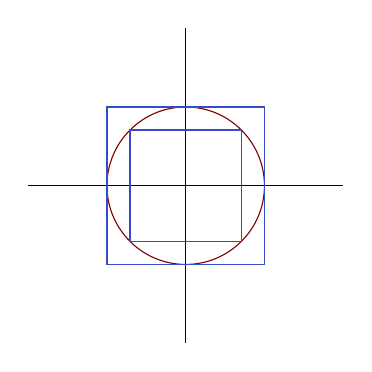
\begin{tikzpicture}
      \draw (-2, 0) -- (2, 0);
      \draw (0, -2) -- (0, 2);
      \draw [mred] circle [radius=1];
      \draw [mblue] (-1, -1) rectangle (1, 1);
      \draw [mblue] (-0.707, -0.707) rectangle (0.707, 0.707);
    \end{tikzpicture}
  \end{center}
  where the blue ones are the balls with respect to $\|\cdot \|_\infty$ and the red one is the ball with respect to $\|\cdot \|_2$.

  In general, we can consider $\R^n$, again with $\|\cdot \|_2$ and $\|\cdot \|_\infty$. We have
  \[
    \|\mathbf{x}\|_\infty \leq \|\mathbf{x}\|_2 \leq \sqrt{n}\|\mathbf{x}\|_\infty.
  \]
\end{eg}
These are easy to check manually. However, later we will show that in fact, any two norms on a finite-dimensional vector space are Lipschitz equivalent. Hence it is more interesting to look at infinite dimensional cases.

\begin{eg}
  Let $V = C([0, 1])$ with the norms
  \[
    \|f\|_1 = \int_0^1 |f|\;\d x,\quad \|f\|_\infty = \sup_{[0, 1]}|f|.
  \]
  We clearly have the bound
  \[
    \|f\|_1 \leq \|f\|_\infty.
  \]
  However, there is no constant $b$ such that
  \[
    \|f\| \leq b\|f\|_1
  \]
  for all $f$. This is easy to show by constructing a sequence of functions $f_n$ by
  \begin{center}
    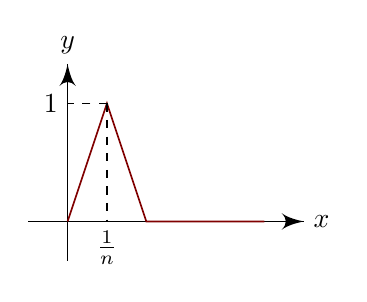
\begin{tikzpicture}
      \draw [->] (-0.5, 0) -- (3, 0) node [right] {$x$};
      \draw [->]  (0, -0.5)  -- (0, 2) node [above] {$y$};
      \draw [mred, semithick] (0, 0) -- (0.5, 1.5) -- (1, 0) -- (2.5, 0);
      \draw [dashed] (0.5, 1.5) -- +(-0.5, 0) node [left] {$1$};
      \draw [dashed] (0.5, 1.5) -- +(0, -1.5) node [below] {$\frac{1}{n}$};
    \end{tikzpicture}
  \end{center}
  where the width is $\frac{2}{n}$ and the height is $1$. Then $\|f_n\|_\infty = 1$ but $\|f_n\|_1 = \frac{1}{n} \to 0$.
\end{eg}
\begin{eg}
  Similarly, the space $\ell^2 = \left\{(x_n): \sum x_n^2 < \infty\right\}$ under the regular $\ell^2$ norm and the $\ell^\infty$ norm, we have
  \[
    \|(x_k)\|_\infty \leq \|(x_k)\|_{\ell^2},
  \]
  but there is no $b$ such that
  \[
    \|(x_k)\|_{\ell^2} \leq b\|(x_k)\|_\infty.
  \]
  For example, we can consider the sequence $x^n = (1, 1, \cdots, 1, 0, 0, \cdots)$, where the first $n$ terms are $1$.
\end{eg}
So far in all our examples, out of the two inequalities, one holds and one does not. Is it possible for both inequalities to not hold? The answer is yes. This is an exercise on the second example sheet as well.

This is all we are going to say about Lipschitz equivalence. We are now going to define convergence, and study the consequences of Lipschitz equivalence to convergence.
\begin{defi}[Bounded subset]
  Let $(V, \|\cdot \|)$ be a normed space. A subset $E \subseteq V$ is \emph{bounded} if there is some $R > 0$ such that
  \[
    E \subseteq B_R(\mathbf{0}).
  \]
\end{defi}

\begin{defi}[Convergence of sequence]
  Let $(V, \|\cdot\|)$ be a normed space. A sequence $(x_k)$ in $V$ \emph{converges to} $\mathbf{x} \in V$ if $\|\mathbf{x}_k - \mathbf{x}\| \to 0$ (as a sequence in $\R$), ie.
  \[
    (\forall \varepsilon > 0)(\exists N)(\forall k \geq N)\; \|\mathbf{x}_k - \mathbf{x}\| < \varepsilon.
  \]
\end{defi}
These two definitions, obviously, depends on the chosen norm, not just the vector space $V$. However, if two norms are equivalent, then they agree on what is bounded and what converges.
\begin{prop}
  If $\|\cdot \|$ and $\|\cdot \|'$ are Lipschitz equivalent norms on a vector space $V$, then
  \begin{enumerate}
    \item A subset $E\subseteq V$ is bounded with respect to $\|\cdot \|$ if and only if it is bounded with respect to $\|\cdot \|'$.
    \item A sequence $x_k$ converges to $x$ with respect to $\|\cdot \|$ if and only if it converges to $x$ with respect to $\|\cdot \|'$.
  \end{enumerate}
\end{prop}

\begin{proof}\leavevmode
  \begin{enumerate}
    \item This is direct from definition of equivalence.
    \item Say we have $a, b$ such that $a\|\mathbf{y}\|  \leq \|\mathbf{y}\|' \leq b\|\mathbf{y}\|$ for all $\mathbf{y}$.  So
      \[
        a\|\mathbf{x}_k - \mathbf{x}\|  \leq \|\mathbf{x}_k - \mathbf{x}\|' \leq b\|\mathbf{x}_k - \mathbf{x}\|.
      \]
      So $\|\mathbf{x}_k - \mathbf{x}\| \to 0$ if and only if $\|\mathbf{x}_k - \mathbf{x}\|' \to 0$. So done.
  \end{enumerate}
\end{proof}
What if the norms are not equivalent? It is not surprising that there are some sequences that converge with respect to one norm but not another. More surprisingly, it is possible that a sequence converges to different limits under different norms. This is, again, on the second example sheet.

We have some easy facts about convergence:
\begin{prop}
  Let $(V, \|\cdot \|)$ be a normed space. Then
  \begin{enumerate}
    \item If $\mathbf{x}_k \to \mathbf{x}$ and $\mathbf{x}_k \to \mathbf{y}$, then $\mathbf{x} = \mathbf{y}$.
    \item If $\mathbf{x}_k \to \mathbf{x}$, $\mathbf{y}_k \to \mathbf{y}$, then $a\mathbf{x}_n \to a\mathbf{x}$ and $\mathbf{x}_k + \mathbf{y}_k \to \mathbf{x} + \mathbf{y}$.
  \end{enumerate}
\end{prop}

\begin{proof}\leavevmode
  \begin{enumerate}
    \item $\|\mathbf{x} - \mathbf{y}\| \leq \|\mathbf{x} - \mathbf{x}_k\| + \|\mathbf{x}_k - \mathbf{y}\| \to 0$. So $\|\mathbf{x} - \mathbf{y}\| = 0$. So $\mathbf{x} = \mathbf{y}$.
    \item Easy exercise.
  \end{enumerate}
\end{proof}
\end{document}
